\documentclass[11pt,a4paper]{article}
\usepackage[utf8]{inputenc}
\usepackage[english]{babel}
\usepackage{amsmath}
\usepackage{amsfonts}
\usepackage{amssymb}
\usepackage{graphicx}
\usepackage{lmodern}
\usepackage{xspace}
\usepackage[colorlinks=true]{hyperref}
\usepackage{tikz}
\usepackage{mytikz}

\usepackage[left=2cm,right=2cm,top=2cm,bottom=2cm]{geometry}

\author{Florian Rabe, Jonas Betzendahl\\(Illustrations by Katja Berčič)}
\title{MMT Internals\\ An Ongoing Tutorial}

\newcommand{\MMT}{\textsf{MMT}\xspace}
\parindent0pt

\begin{document}
\maketitle
{\hypersetup{hidelinks}\tableofcontents}
\bigskip

\section{Introduction}



\newpage
\section{Overview (2018-11-28/29)}
\label{sec:overview}

\textbf{Full session on YouTube:} \href{https://www.youtube.com/watch?v=PUKjQbbeqdQ}{Part 1}, \href{https://www.youtube.com/watch?v=yh_vwVm8Szc}{Part 2}.

\subsection{Structural Elements and Objects}

\textbf{Further reading:} \href{https://uniformal.github.io/doc/language/}{Structure}
\bigskip

All \MMT content is divided into the \emph{structure level} and the \emph{object level} (compare Figure \ref{fig:mmtcontent}). The structure level is a tree of so-called structural elements (see the corresponding class, \href{https://uniformal.github.io/apidoc/info/kwarc/mmt/api/StructuralElement.html}{\texttt{StructuralElement}}) that all have a path (\emph{D}ocuments have a \texttt{DPath}, \emph{M}odules have an \texttt{MPath} and Declarations have a \texttt{GlobalName}; the latter two also have a name, which is a \texttt{LocalName}).

The general idea is that documents (everything from a repository to a directory to a file to a section within a file can be viewed as a document here) contain lists of modules and modules contain lists of declarations. Both modules and documents can also contain  other modules or documents respectively. Narrative structure of documents (what files are in what directories etc.) does not carry any semantics. For this, modules should be used instead.

\begin{figure}[h]
\centering
\begin{tikzpicture}[xscale=.9]

\node (content) at (0,0) {MMT Content};

\node (obj) at (5.5,-1) {Object Level};
\draw[arrow] (content) -- (obj);
\node (struct) at (-5,-1) {Structure Level};
\draw[arrow] (content) -- (struct);

\node (notation) at (9,-2) {Notation};
\draw[arrow] (obj) -- (notation);
\node (term) at (7,-2) {Term};
\draw[arrow] (obj) -- (term);
\node (sub) at (4.5,-2) {Substitution};
\draw[arrow] (obj) -- (sub);
\node (context) at (1.5,-2) {Context};
\draw[arrow] (obj) -- (context);

\node (doc) at (-7.5,-2) {Document};
\draw[arrow] (struct) -- (doc);
\node (mod) at (-5,-2) {Module};
\draw[arrow] (struct) -- (mod);
\node (decl) at (-2.5,-2) {Declaration};
\draw[arrow] (struct) -- (decl);
 
\end{tikzpicture}
\caption{Overview of content structure. Nodes in this tree generally correspond to Scala classes.}
\label{fig:mmtcontent}
\end{figure}

The prominent examples for modules would be \href{https://uniformal.github.io/doc/language/modules.html#theories}{theories} or \href{https://uniformal.github.io/doc/language/modules.html#views}{views} and for declarations \href{https://uniformal.github.io/doc/language/declarations.html#constants}{constants}. These in terms have components that are objects. For example, theories have metatheories, views have domains and codomains, and constants have any number of types, definition and notations, which are all \emph{terms}.

The following is a good first overview about what forms \MMT terms take (for more on this, also see Section \ref{sec:terms}, where the object level is discussed in more detail):

\begin{itemize}
\item \textbf{OMS}\\ (OpenMath Symbol, refers to a constant)
\item \textbf{OMA}\\ (OpenMath Application, takes operator/function and children/arguments)
\item \textbf{OMBIND}\\ (OpenMath Binder, binds variables)
\item \textbf{OMV}\\ (OpenMath Variable)
\item \textbf{OMLIT}\\ (OpenMath Literals)
\end{itemize}

\subsection{Algorithms}

\MMT 's architecture has three phases. These correspond most interesting and relevant algorithms \MMT offers, which will we be discussing next. The three phases are:

\begin{itemize}
\item \textbf{Lexing / Parsing}\\ (no real distinction, we'll refer to this as just ``parsing'' from now on)
\item \textbf{Type Checking}\\ (this includes type inference and type reconstruction)
\item \textbf{Simplification}\\ (this also includes elaboration)
\end{itemize}

Each of these phases is called on each declaration separately and the first declaration is entirely processed (through all three phases) before the second declaration is touched. It is \emph{not} the case that \MMT first parses everything, then typechecks everything and finally simplifies everything. This is so  because the successful processing of a later declaration might depend on the complete result of an earlier declaration (imagine a \href{https://uniformal.github.io/doc/language/declarations.html#notations}{notation} being used that was only introduced earlier in the file).
\bigskip

The code equivalent to these algorithms are also separated along the same divide of object- and structure-level. So the \MMT API contains Scala classes like \texttt{StructureParser}, \texttt{StructureChecker} and \texttt{StructureSimplifier} as well as \texttt{ObjectParser}, \texttt{ObjectChecker} and \texttt{ObjectSimplifier}. 

\texttt{StructureX}s take \texttt{ObjectX}s as arguments, to ensure modularity. For example, you could probably write an entirely new StructureParser in an afternoon, that you could then use with the already existing object parser without any problems. 

Any \href{https://uniformal.github.io/doc/setup/#2-install-an-ide-jedit-or-intellij-idea-if-you-havent-already}{IDE} features are built on top of this, meaning that any new component here could also easily be used for development in IDEs.

\begin{figure}[ht]
\centering
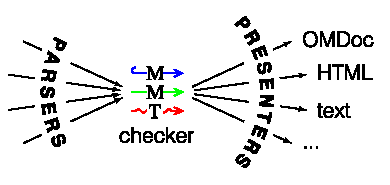
\includegraphics[scale=1.5]{parsers-mmt-presenters.pdf}
\caption{There can be many parsers and many presenters, but they all use the same \MMT checker}
\label{fig:mmtbottleneck}
\end{figure}

As a general rule, the pipeline flow is many to one to many (compare Figure \ref{fig:mmtbottleneck}). There are multiple parsers and presenters (like HTML, plaintext, \dots) and you could relatively easily add your own (if you would like a parser that is more suitable to your particular needs, like, say, one that parses JSON). However, every instantiation  of the pipeline uses the same \MMT checker.

The standard classes for each of these is given in the table in Figure \ref{tbl:standardnames}.

\begin{figure}[ht]
\centering
\begin{tabular}{ |c|c|c| } 
 \hline
 & \textbf{Structure}: & \textbf{Object}: \\
 \hline
 \textbf{Parsing}: & \href{https://uniformal.github.io/apidoc/info/kwarc/mmt/api/parser/KeywordBasedParser.html}{\texttt{KeywordBasedParser}} & \href{https://uniformal.github.io/apidoc/info/kwarc/mmt/api/parser/NotationBasedParser.html}{\texttt{NotationBasedParser}} \\ 
 \textbf{Checking}: & \href{https://uniformal.github.io/apidoc/info/kwarc/mmt/api/checking/MMTStructureChecker.html}{\texttt{MMTStructureChecker}} & \href{https://uniformal.github.io/apidoc/info/kwarc/mmt/api/checking/RuleBasedChecker.html}{\texttt{RuleBasedChecker}} \\ 
 \textbf{Simplifying}: & \href{https://uniformal.github.io/apidoc/info/kwarc/mmt/api/uom/ElaborationBasedSimplifier.html}{\texttt{ElaborationBasedSimplifier}} & \href{https://uniformal.github.io/apidoc/info/kwarc/mmt/api/uom/RuleBasedSimplifier.html}{\texttt{RuleBasedSimplifier}} \\ 
 \hline
\end{tabular}
\caption{Standard Names}
\label{tbl:standardnames}
\end{figure}

In the following sections, we will take a closer look at each of the three main phases.

\subsubsection{Parsing}

\textbf{Further reading:} \href{https://uniformal.github.io/doc/language/delimiters.html}{Delimiters}
\bigskip

Parsing in \MMT is usually (if you don't roll your own differently) done with delimiters and keyword. Everything starts with a keyword and ends with a delimiter. If you've written some \MMT surface syntax, you will be already familiar with these delimiters.

This structure can also easily be nested.

The most important delimiters (not bothering with document delimiters) are:

\begin{itemize}
\item \texttt{MD} (Module Delimiter)
\item \texttt{DD} (Declaration Delimiter)
\item \texttt{OD} (Object Delimiter)
\end{itemize}

There are two classes, \texttt{ParsingStream} and \texttt{ParsingUnit}, which encapsulate just about everything you conceivably would want to parse.
\subsubsection{Type Checking}
\subsubsection{Simplification}

\newpage
\section{Terms (2019-01-31)}
\label{sec:terms}

\textbf{Full session on YouTube:} \href{https://www.youtube.com/watch?v=vtePl2pGhfc}{Link}.
\bigskip

\begin{figure}[ht]
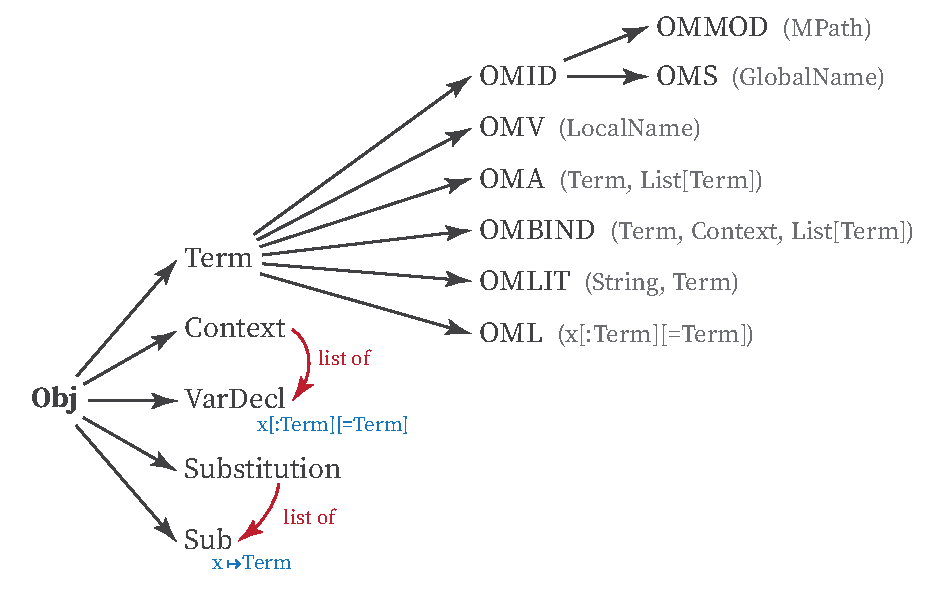
\includegraphics[scale=1]{mmt-terms.pdf}
\caption{Overview of \MMT Terms}
\label{fig:mmtterms}
\end{figure}


\end{document}